\documentclass[11pt,psfig]{article}
\usepackage{epsfig}
\usepackage{times}
\usepackage{amssymb}
\usepackage{float}
\usepackage{listings}
\usepackage{graphicx}
\usepackage{caption}
\usepackage{subcaption}

\newcount\refno\refno=1
\def\ref{\the\refno \global\advance\refno by 1}
\def\ux{\underline{x}}
\def\uw{\underline{w}}
\def\bw{\underline{w}}
\def\ut{\underline{\theta}}
\def\umu{\underline{\mu}} 
\def\bmu{\underline{\mu}} 
\def\be{p_e^*}
\newcount\eqnumber\eqnumber=1
\def\eq{\the \eqnumber \global\advance\eqnumber by 1}
\def\eqs{\eq}
\def\eqn{\eqno(\eq)}

 \pagestyle{empty}
\def\baselinestretch{1.1}
\topmargin1in \headsep0.3in
\topmargin0in \oddsidemargin0in \textwidth6.5in \textheight8.5in
\begin{document}
\setlength{\parskip}{1.2ex plus0.3ex minus 0.3ex}


\thispagestyle{empty} \pagestyle{myheadings} \markright{Homework
2: CS 217 Spring 2015}



\title{CS 217 Homework 3}
\author{Zachary DeStefano, 15247592}
\date{Due Date: May 26, 2015}

\maketitle

\vfill\eject

\newpage

\section*{Problem 1}

\subsection*{Part 1}

If $L$ is the direction of the light source, $N$ is the normal to the surface, we know that the intensity of the light $I$ is given by
\[
I = |L| |N| cos(\alpha)
\]
where $\alpha$ is the angle between $L$ and $N$.\\
That equation is maximized when $cos(\alpha)=1$ so that $\alpha=0$\\
This means that the normal is pointing in the direction of the light source. \\
Thus the light source is in the direction of $(a,b)$.\\
To find the corresponding point on the sphere, we need to find $c$ such that $a^2 + b^2 + c^2 = r^2$\\
\\
Since we are projecting the sphere onto the x-y plane, we are going to see the positive side, thus we will use the positive solution to the above equation. Thus our point on the sphere is as follows:
\[
(a,b,\sqrt{r^2-(a^2+b^2)})
\]
That vector has magnitude $r$ thus the unit vector for this point that points in the direction of the light source is as follows:
\[
(\frac{a}{r},\frac{b}{r},\frac{\sqrt{r^2-(a^2+b^2)}}{r})
\]

\newpage

\subsection*{Part 2}

Let $L$ be the direction of the light from $(a,b,c)$, \\
$N$ be the normal to the surface at $(a,b,c)$, and \\
$E$ be the vector pointing from $(a,b,c)$ to the viewer. \\
\\
$L$ will be the reflection vector of $E$ from the surface with normal $N$ since we have specular reflection\\
As illustrated below it will hold that
\[
L + E = 2N(E \cdot N)
\]
Thus we have the formula for $L$
\[
L = 2N(E \cdot N) - E
\]
\begin{figure}[H]
\centering
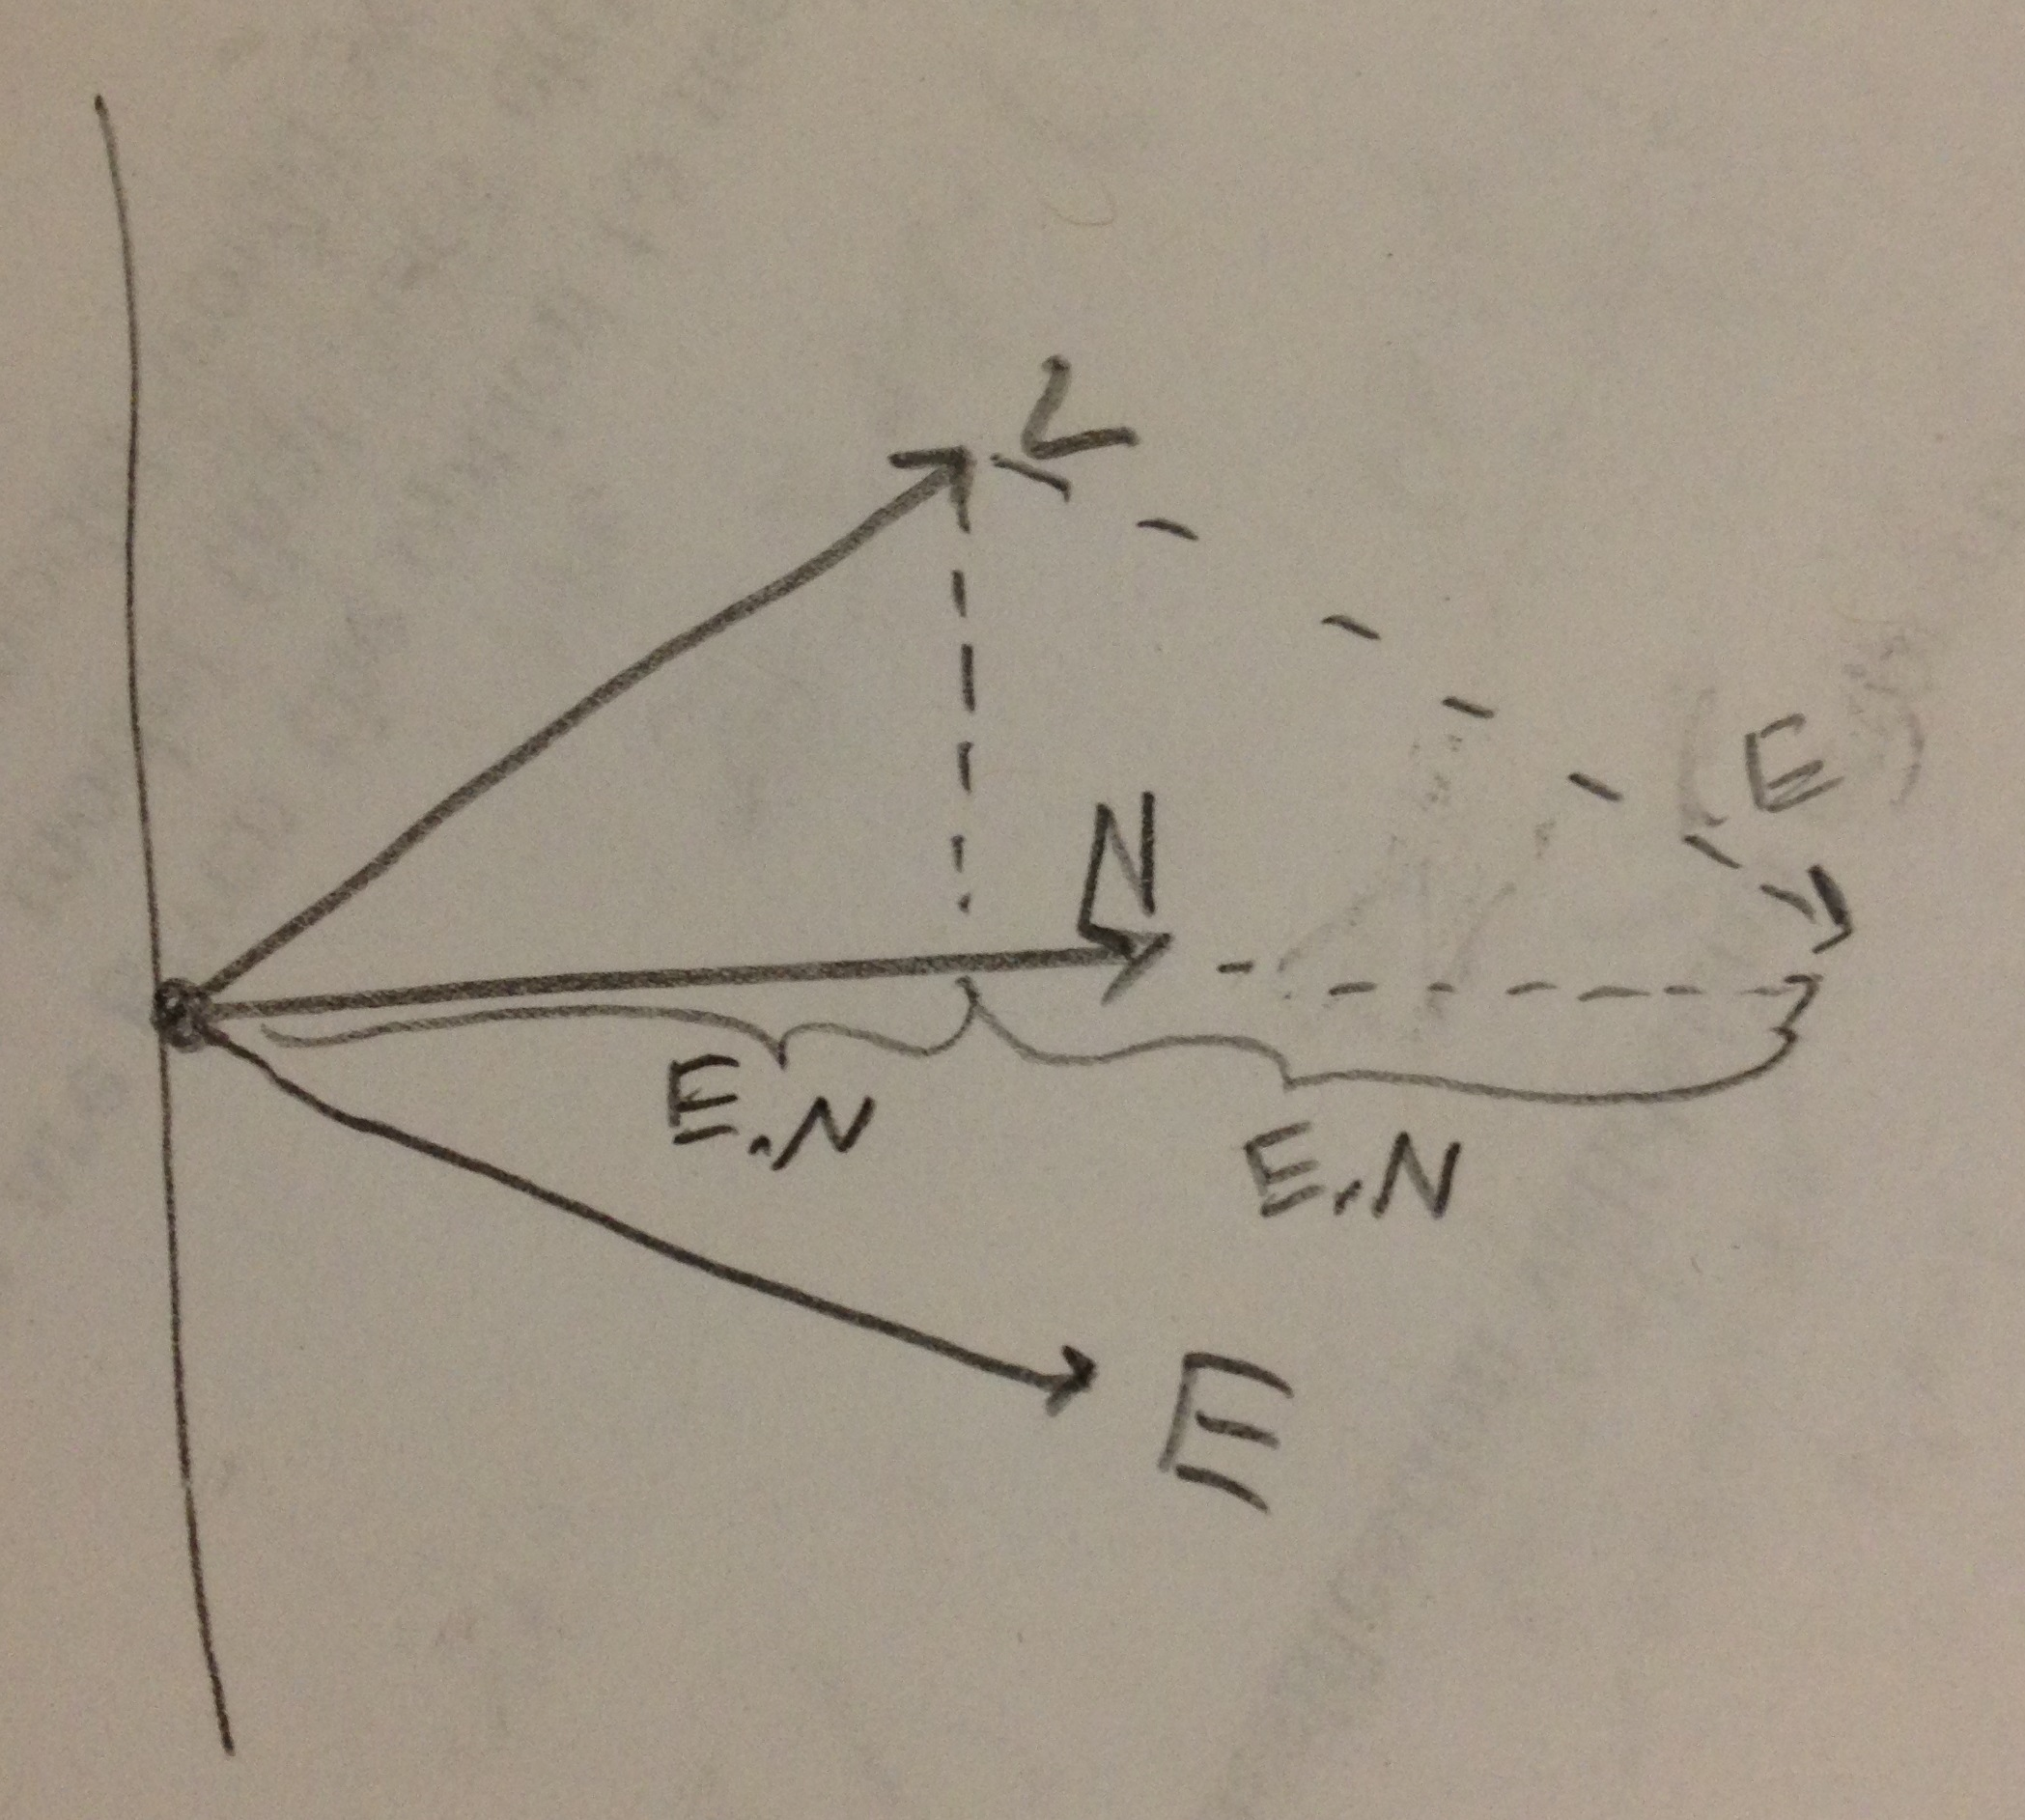
\includegraphics[height=3.5in]{prob1diagram.jpg}
\caption{Illustration of normal vector N, light vector L, and viewing vector E and their relationships}
\end{figure}

\newpage

E is parallel to the viewing direction thus \\
$E=(0,0,1)$\\
$N = \frac{1}{r}(a,b,c)$\\
We can thus say that $E \cdot N = \frac{c}{r}$, finally letting us say that
\[
L = (\frac{2ac}{r^2},\frac{2bc}{r^2},\frac{2c^2}{r^2} - 1)
\]
Now it holds that
\[
||L||_2^2 = \frac{4a^2c^2 + 4b^2c^2 + 4c^4 - 4r^2c^2 + r^4}{r^4}
\]
Factoring out $4c^2$ gives us
\[
||L||_2^2 = \frac{4c^2(a^2 + b^2 + c^2 - r^2) + r^4}{r^4}
\]
We know that $r^2 = a^2 + b^2 + c^2$ thus finally $||L||_2^2 = 1$\\
Proving that $L$ is a unit vector and thus in its final form

\newpage

\section*{Problem 2}

For the images 1 to 11, here are the normal vectors in order at the bright spot, which would be the lighting direction if the sphere were diffuse. Each row indicates a vector in order $(x,y,z)$ 
\begin{verbatim}
N =

   -0.0672    0.1261    0.9897
   -0.0924   -0.0168    0.9956
   -0.2269   -0.0504    0.9726
   -0.2689   -0.1681    0.9484
   -0.2941   -0.0588    0.9540
   -0.2185    0.1513    0.9640
   -0.2269    0.0504    0.9726
   -0.1681    0.1092    0.9797
   -0.1681    0.0504    0.9845
   -0.0252    0.0672    0.9974
   -0.1849   -0.0672    0.9805
\end{verbatim}

Here are the lighting directions $L$ for images 1 to 11 with the sphere being chrome and specular. The format for specifying vectors is the same as above.

\begin{verbatim}
L =

   -0.1331    0.2495    0.9592
   -0.1841   -0.0335    0.9823
   -0.4414   -0.0981    0.8920
   -0.5101   -0.3188    0.7989
   -0.5612   -0.1122    0.8201
   -0.4213    0.2916    0.8588
   -0.4414    0.0981    0.8920
   -0.3293    0.2141    0.9196
   -0.3309    0.0993    0.9384
   -0.0503    0.1341    0.9897
   -0.3625   -0.1318    0.9226
\end{verbatim}

The code that I used to compute this is attached in prob2script.m

\newpage

\section*{Problem 3}

Here are a few of the needle diagrams with the owl images. The value I obtain for $\rho_r$ is 0.5471. The code to compute it is attached in prob3script.m.

\begin{figure}[H]
\centering
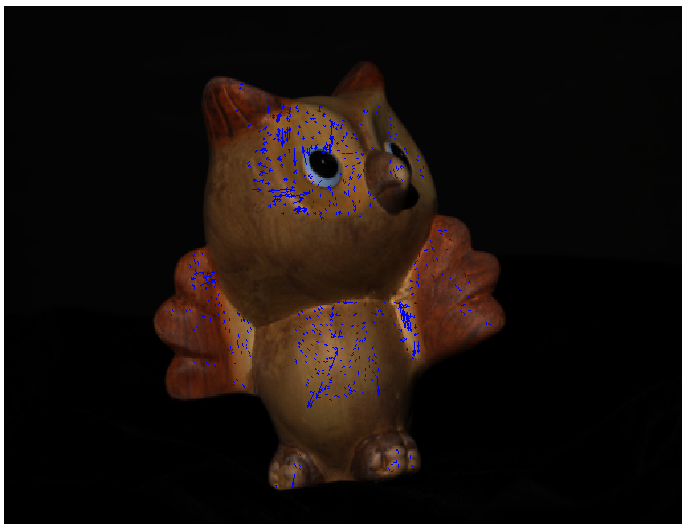
\includegraphics[height=3.5in]{prob3figure1.png}
\end{figure}
\begin{figure}[H]
\centering
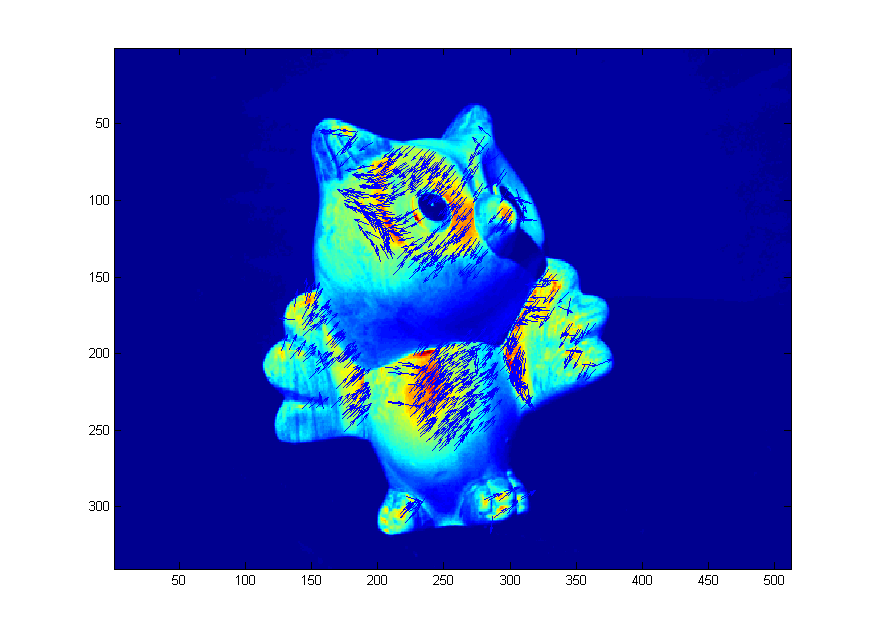
\includegraphics[height=3.5in]{prob3figure2.png}
\end{figure}
\begin{figure}[H]
\centering
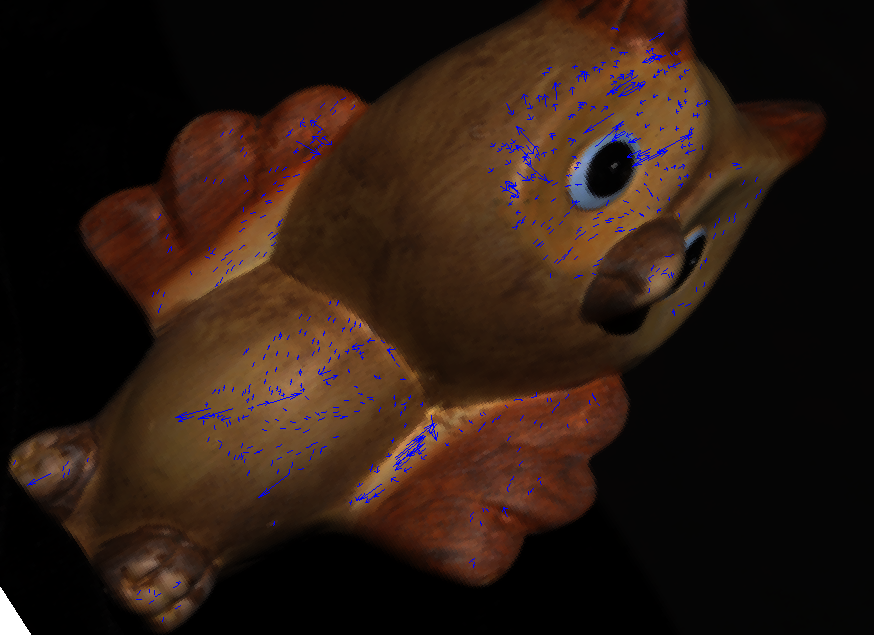
\includegraphics[height=3.5in]{prob3figure3.png}
\end{figure}
\begin{figure}[H]
\centering
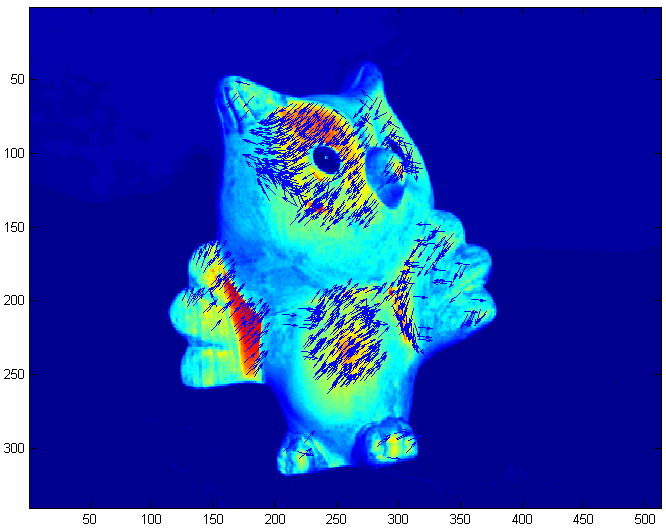
\includegraphics[height=3.5in]{prob3figure4.png}
\end{figure}
\begin{figure}[H]
\centering
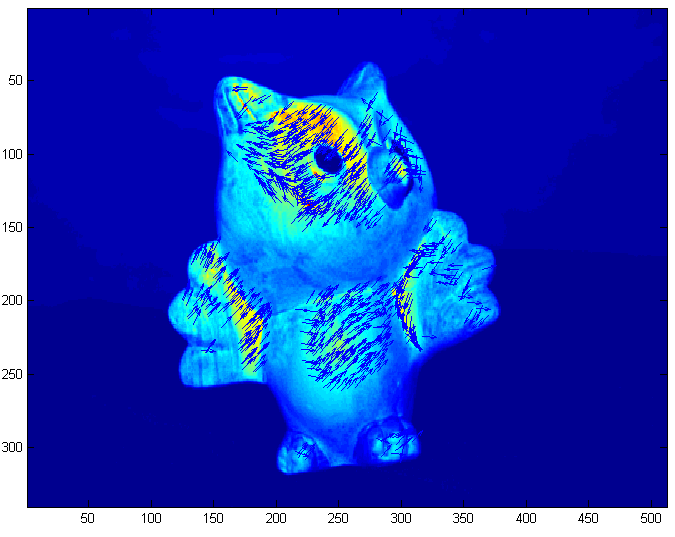
\includegraphics[height=3.5in]{prob3figure5.png}
\end{figure}

\newpage

\section*{Problem 4}

I found the following average $\rho$ values for this problem\\
$\rho_r = 0.5471$\\
$\rho_g = 0.6722$\\
$\rho_b = 0.6722$\\
\\
The code to compute everything is in prob4script.m. It is mostly the same as the code from Problem 3, except that I vary the color channel selection. \\
\\
Here are the needle diagrams for this problem. As can be observed, the normals point in roughly the same direction when a pixel has a normal in multiple channels. 
\begin{figure}[H]
\centering
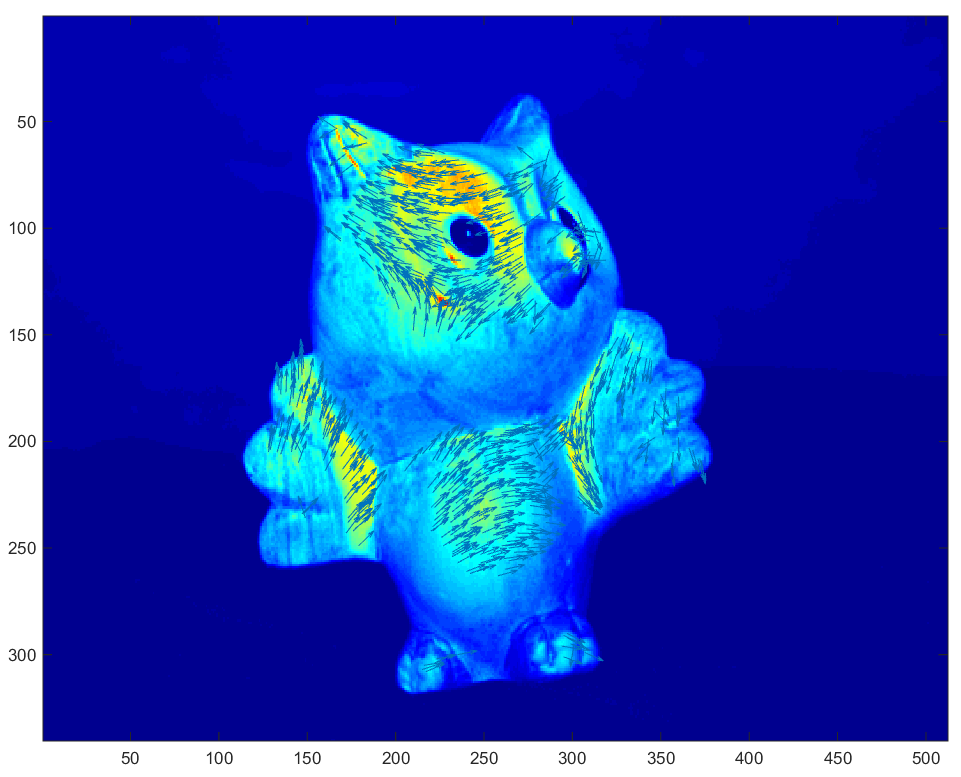
\includegraphics[height=5.5in]{prob4needlePlot1.png}
\caption{Needle Diagram for Red Channel}
\end{figure}
\begin{figure}[H]
\centering
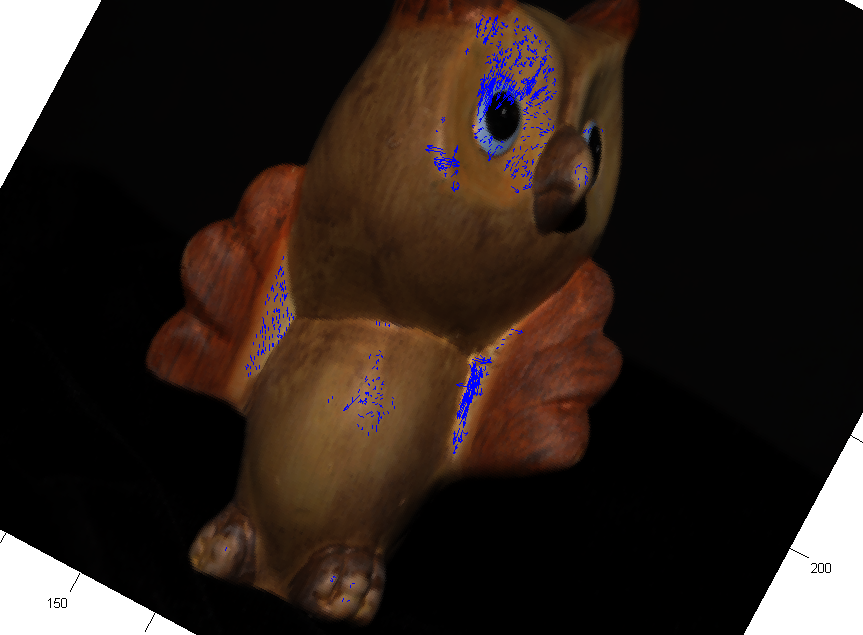
\includegraphics[height=5.5in]{prob4needlePlot2.png}
\caption{Needle Diagram for Green Channel}
\end{figure}
\begin{figure}[H]
\centering
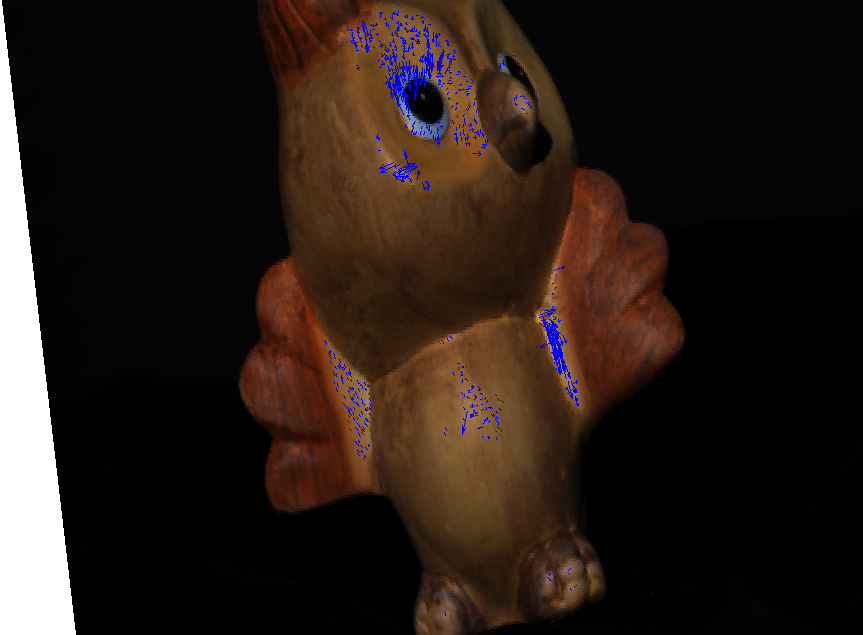
\includegraphics[height=5.5in]{prob4needlePlot3.png}
\caption{Needle Diagram for Blue Channel}
\end{figure}
\newpage
Here are the figures for the $\rho$ values at each pixel with each channel. I set $\rho=0$ if it could not be computed at that pixel.
\begin{figure}[H]
\centering
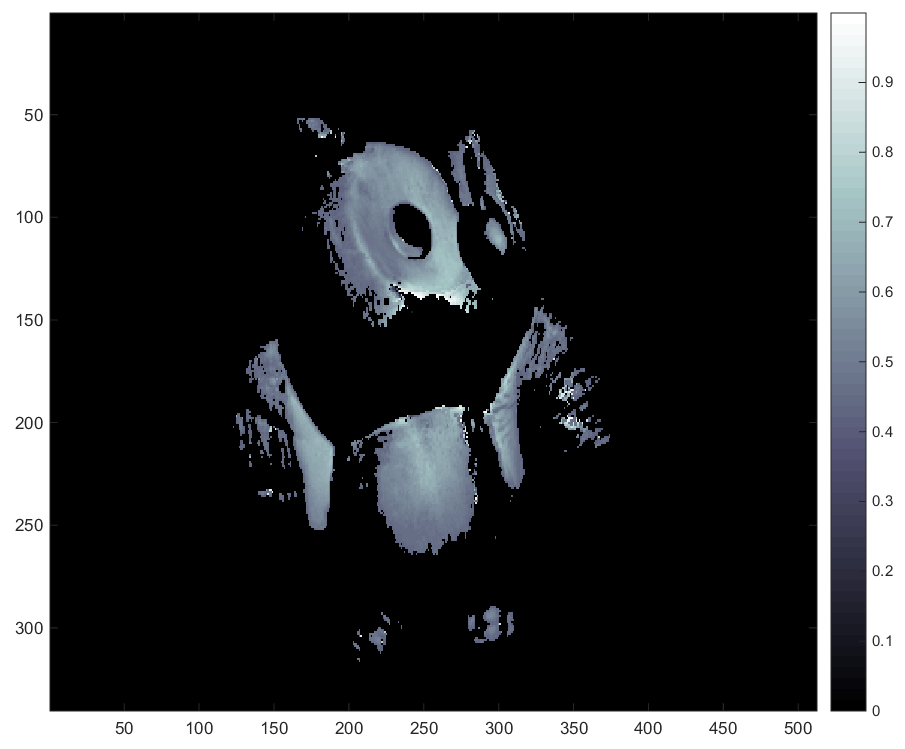
\includegraphics[height=5in]{prob4rhoPlot1.png}
\caption{$\rho$ Plot for Red Channel}
\end{figure}
\begin{figure}[H]
\centering
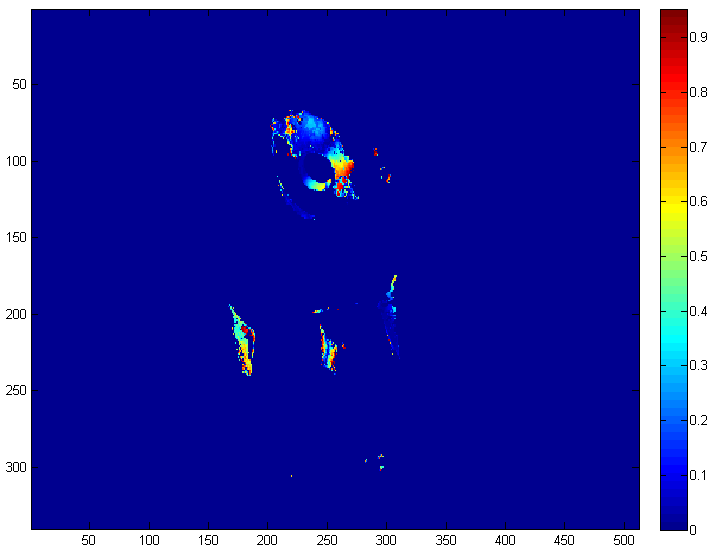
\includegraphics[height=5in]{prob4rhoPlot2.png}
\caption{$\rho$ Plot for Green Channel}
\end{figure}
\begin{figure}[H]
\centering
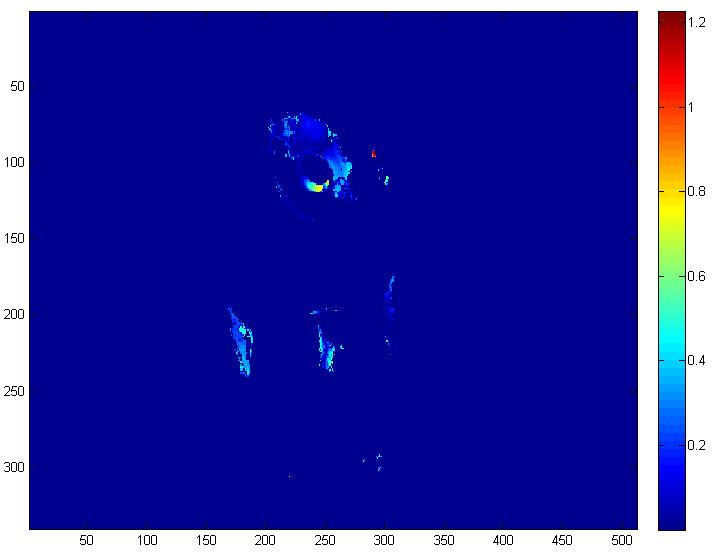
\includegraphics[height=5in]{prob4rhoPlot3.png}
\caption{$\rho$ Plot for Blue Channel}
\end{figure} 


\end{document}








